\documentclass{article}
\usepackage[utf8]{inputenc}
\def\MakeUppercaseUnsupportedInPdfStrings{\scshape}
\usepackage{float}
\usepackage{hyperref}
\usepackage{graphicx}

\title{Aubo Guides and Training material}
\author{Lead Robotics}
\date{May 2022 v0.1.0}

\begin{document}

\maketitle

\tableofcontents

\section{This document}
This document is a manual for setting up the Aubo for the WheelRestore System. 

The required steps to setup a robot for wheelrestore are sections \ref{subsec:statIPsysSett} to \ref{subsec:usingBackup}. 
\begin{enumerate}
\item Set static IP using system settings
\item Update Aubo software via USB
\item Installing Aubo Programs Using Backup File
\end{enumerate}

The rest of the document is either optional or alternative ways of doing these 3 things. 

You will need a USB with the update software. The USB should also have a backup of the demo-machine, you will use to install the robotprograms, setup modbus etc.

\section{Guide}

\subsection{Set static IP using system settings} \label{subsec:statIPsysSett}
\begin{enumerate}
\item Connect the three cables to the controlbox. Connect the other ends to the manipulater arm, 230VAC power and the teacpendant screen respectively.
\item Turn the box on. On the compact box the switch is located right above the power cord plugin. On the large box the breaker is round and jutting out of the front of the box. After turning the switch you should hear the fans start in the box.
\begin{figure}[H]\centering
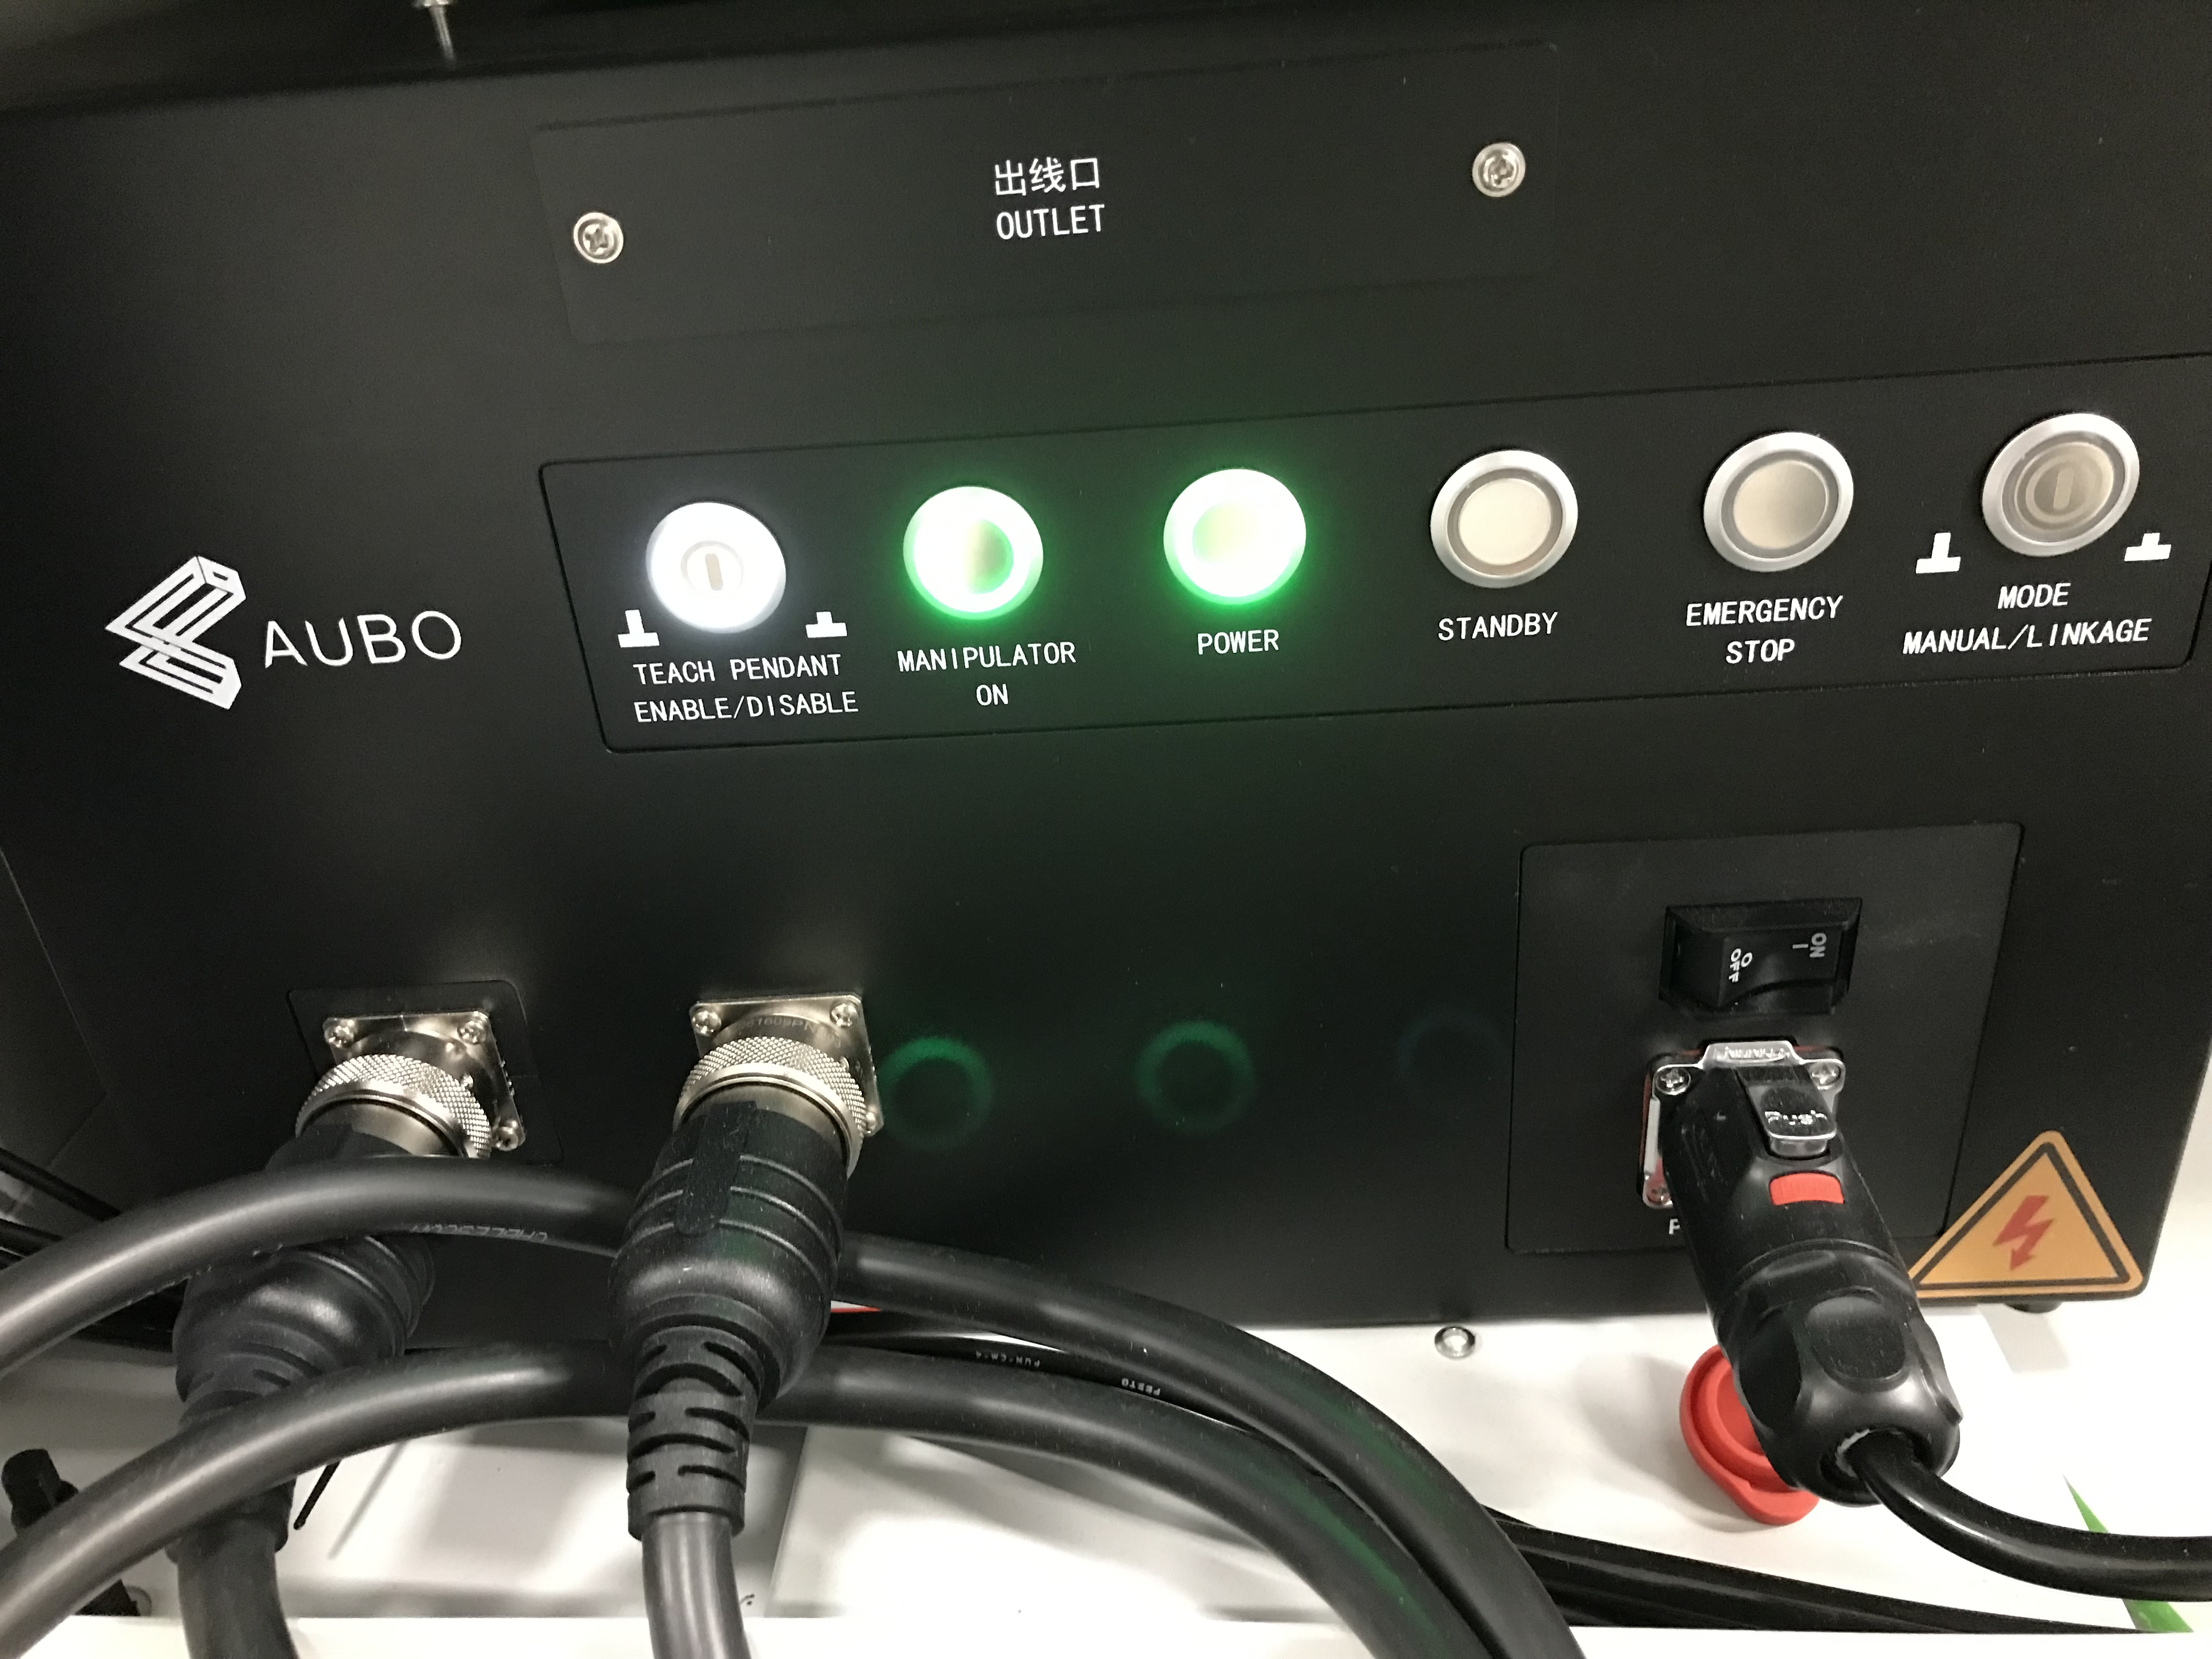
\includegraphics[width=0.8\textwidth]{../../Images/FrontCompactAuboBox.jpg}
\end{figure}
\item Wait for the $Standby$ light to turn on with a solid orange light. 
\item If the Emergency stop light is lit up in red make sure to clear the emergency stop button.
\item Now get the teachpendant and press and hold the power button in the top-left corner for at least 1s. The button should light up blue.
\item Wait for the teachpendant to start. 
\item A guarantee disclaimer might appear, click agree to continue. 
\item You should now see a login screen and a desktop. 
\begin{figure}[H]\centering
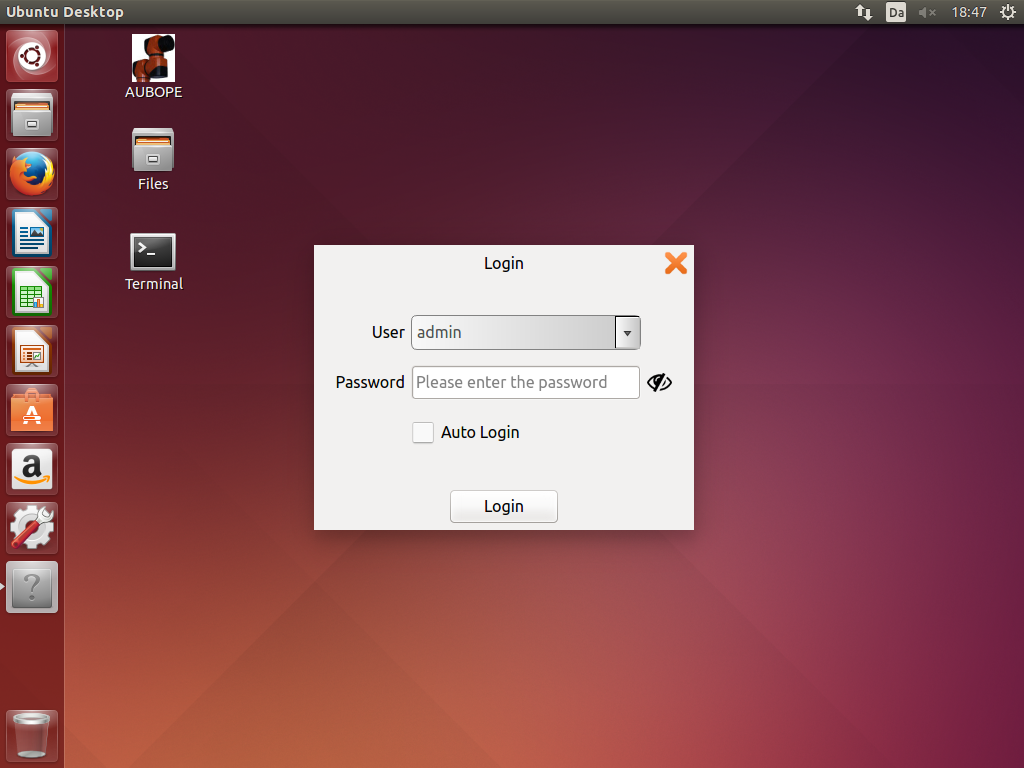
\includegraphics[width=0.8\textwidth]{../../Images/loginScreen.png}
\end{figure}
\item Close the login screen for now, we will get to the robot program later. 
\item You should now only see the desktop with 3 shortcuts: $AUBOPE$, $Files$ and $Terminal$. AUBOPE is the robot software. This will re-open the login screen and get us into the robot programming. Files opens the filesystem. Terminal opens a bash terminal.
\item Open a terminal, by double tapping the icon. (or plug in a mouse and doubleclick on it)
\item  We now need to type a terminal command beware if you haven't changed the keyboard layout the $\&$ sign will be on the key press $Shift+7$ as on a US keyboard not on a keypress of $Shift+6$ as with a Danish keyboard. Enter command: $unity\&$ .
This command will start the unity desktop environment and give you a toolbar on the left side of the screen.
\item Open system settings either on the toolbar to the left or with the dropdown menu in the topright corner of the screen. The icon is a gear and a wrench. 
\begin{figure}[H]\centering
  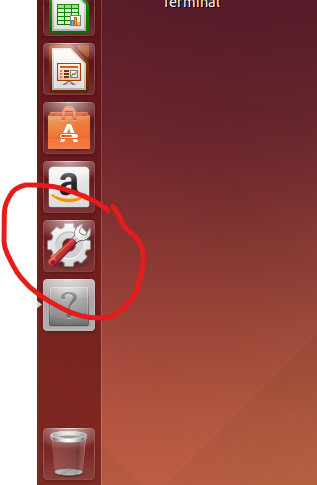
\includegraphics[width=0.3\textwidth]{../../Images/systemSettingsButton.png}
\end{figure}
\begin{figure}[H]\centering
  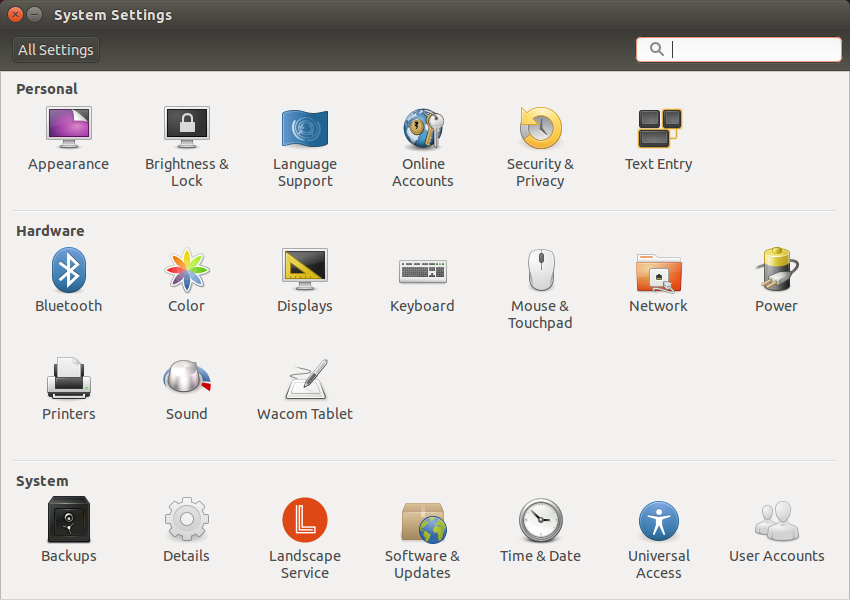
\includegraphics[width=0.8\textwidth]{../../Images/systemSettings.png}
\end{figure}
\item Doubleclick on network
\begin{figure}[H]\centering
  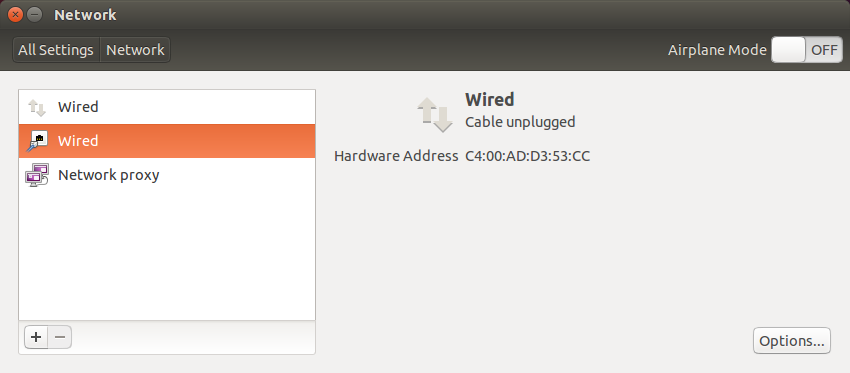
\includegraphics[width=0.8\textwidth]{../../Images/networkWired.png}
\end{figure}
\item Select wired. The icon with the ethernet port not the arrows.
\item click options
\begin{figure}[H]\centering
  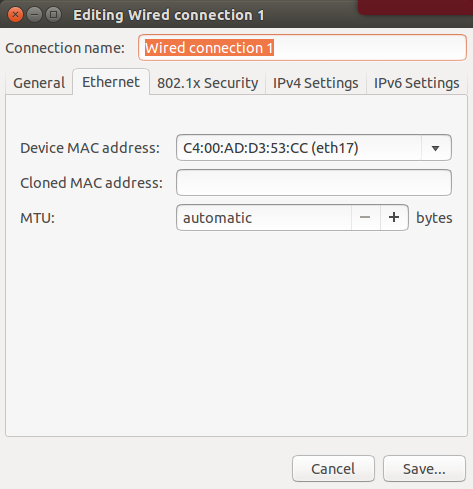
\includegraphics[width=0.8\textwidth]{../../Images/wireOptionsEthernet.png}
\end{figure}
\item Select the IPv4 settings tab
\begin{figure}[H]\centering
  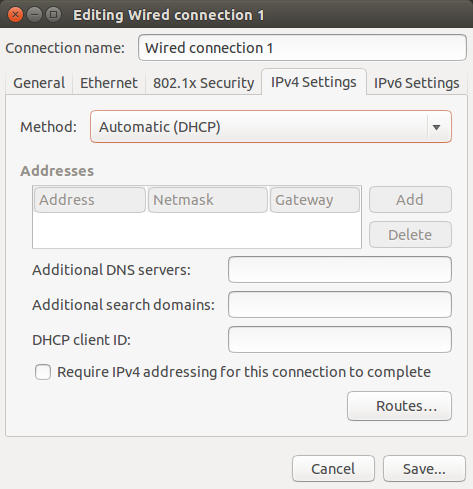
\includegraphics[width=0.8\textwidth]{../../Images/IPv4SettingsAutomatic.png}
\end{figure}
\item In the Method dropdown bar select $'manual'$ 
\begin{figure}[H]\centering
  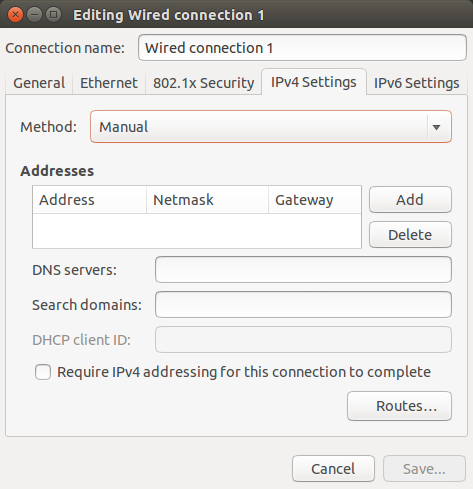
\includegraphics[width=0.8\textwidth]{../../Images/ipv4SettingsManual.png}
\end{figure}
\item Click add and type in IP 192.168.2.41, mask 255.255.255.0 and leave gateway empty. 
\begin{figure}[H]\centering
  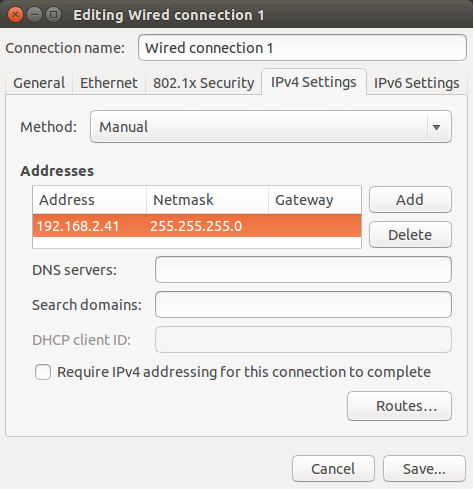
\includegraphics[width=0.8\textwidth]{../../Images/IPv4SettingsWithAdress.png}
\end{figure}
\item Click save. 
\item Close the settings window and the terminal window.  $x$ is in the top left corner of the windows.
\end{enumerate}
The robot should now have a static IP. You can test it by connecting a computer and pinging the robot on its new adress. 



\subsection{Update Aubo software Via USB}
\begin{enumerate}
\item Acquire USB with update software. the software is a compressed file ending in .aubo. 
\item Plugin the usb. 
\item Open AuboPE by double-clicking the shortcut on the desktop
 or by restarting the robot. The login screen should appear.
\begin{figure}[H]\centering
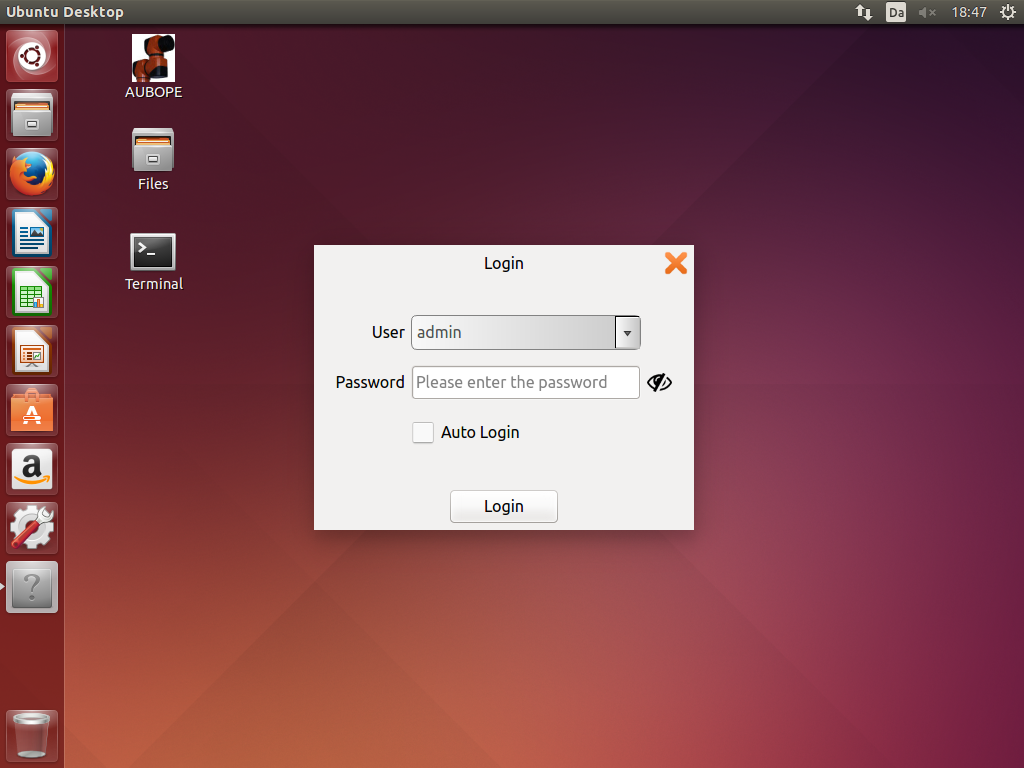
\includegraphics[width=0.8\textwidth]{../../Images/loginScreen.png}
\end{figure}
\item  Type the password, default is '1' and press login. The $Robot Init Form$ screen should appear
\begin{figure}[H]\centering
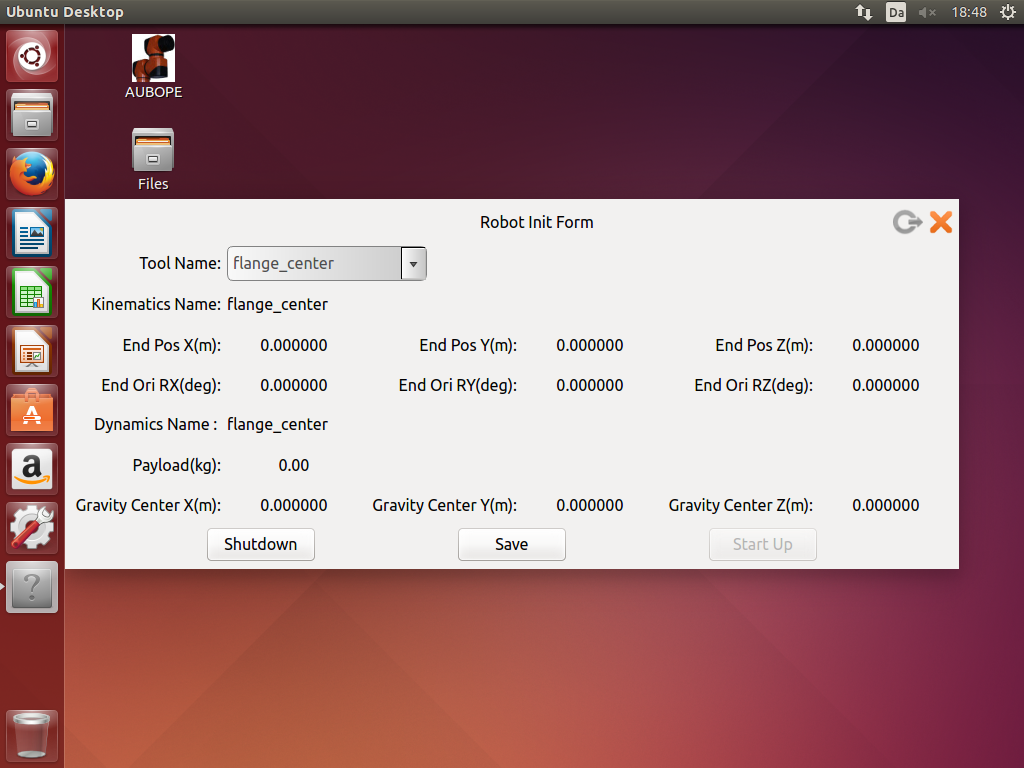
\includegraphics[width=0.8\textwidth]{../../Images/RobotInitForm.png}
\end{figure}
\item Press save and then startup to proceed.If this is the first time the robot has been started after being mounted it will say that the mounting pose has been changed. Click $ok$ and then click $yes$ to confirm that the mounting pose has changed. The robot will now initialize. You should hear the brakes click.  The teachpendant should then show the robot user interface.  
\item Click on the settings tab at the top. 
\begin{figure}[H]\centering
  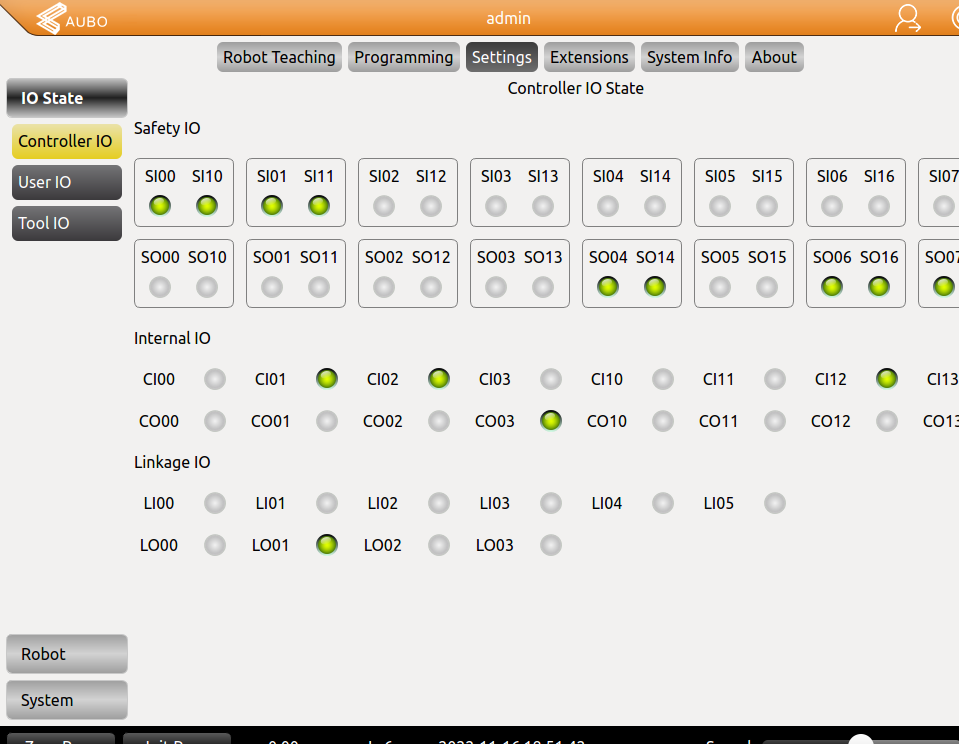
\includegraphics[width=0.8\textwidth]{../../Images/settings.png}
\end{figure}
\item Navigate through the $System$ tab into the $Update$ tab on the bottom left. 
\begin{figure}[H]\centering
  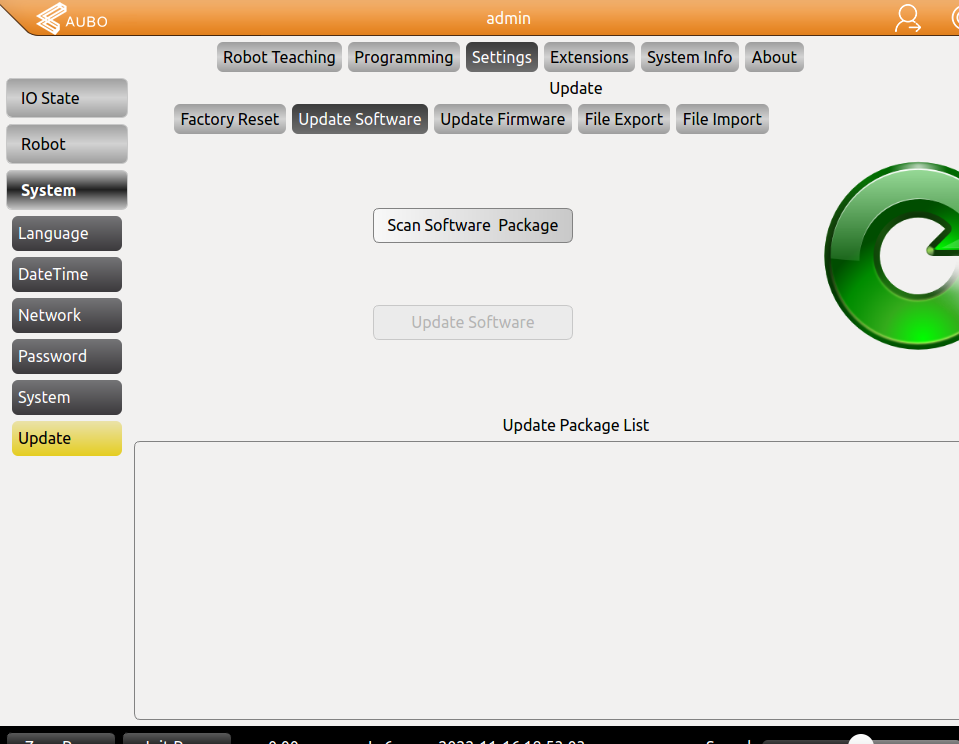
\includegraphics[width=0.8\textwidth]{../../Images/update.png}
\end{figure}
\item Click on the $'Scan Software Package'$ button in the center of the screen. The path to the update file on your USB should appear in the $Update Package List$.
\begin{figure}[H]\centering
  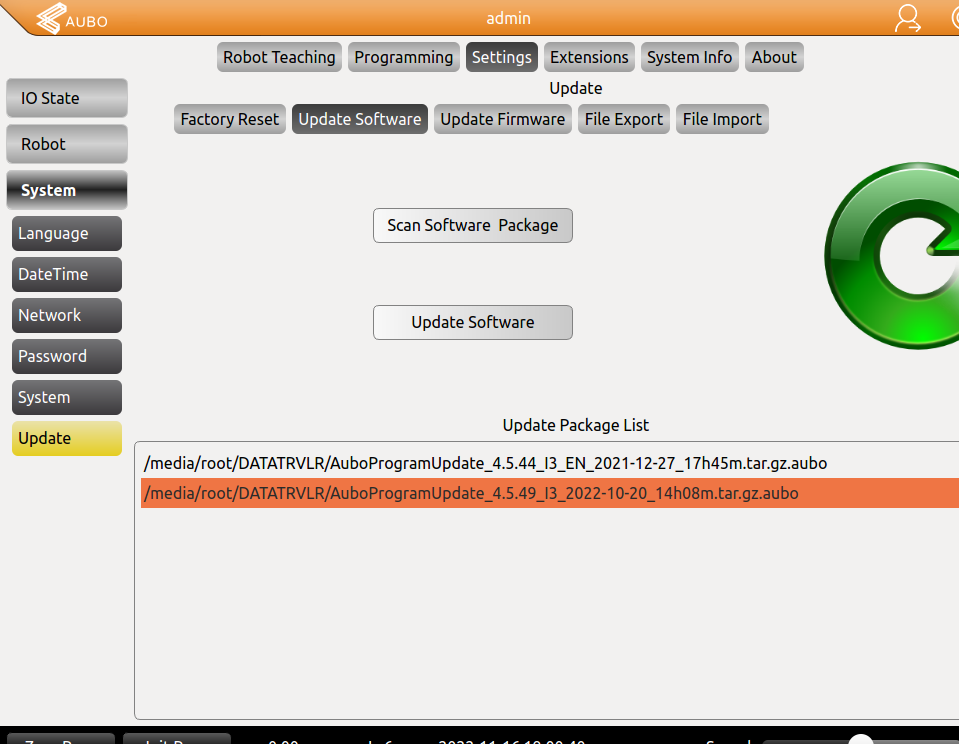
\includegraphics[width=0.8\textwidth]{../../Images/lisrofUpdateFiles.png}
\end{figure}
\item Select your desired update file and press $'Update Software'$
\item A confirmation window will appear. Press $'yes'$ you do want to update.
\item Wait for the update to finish. This will take about 30 seconds. 
\item The program will tell you to restart. Click $'ok'$, and then $'yes'$ to shutdown.
\item Start the robot again with the power button on the teachpendant. The login screen should appear.
\item  Type the password, default is '1' and press login. The $Robot Init Form$ screen should appear
\begin{figure}[H]\centering
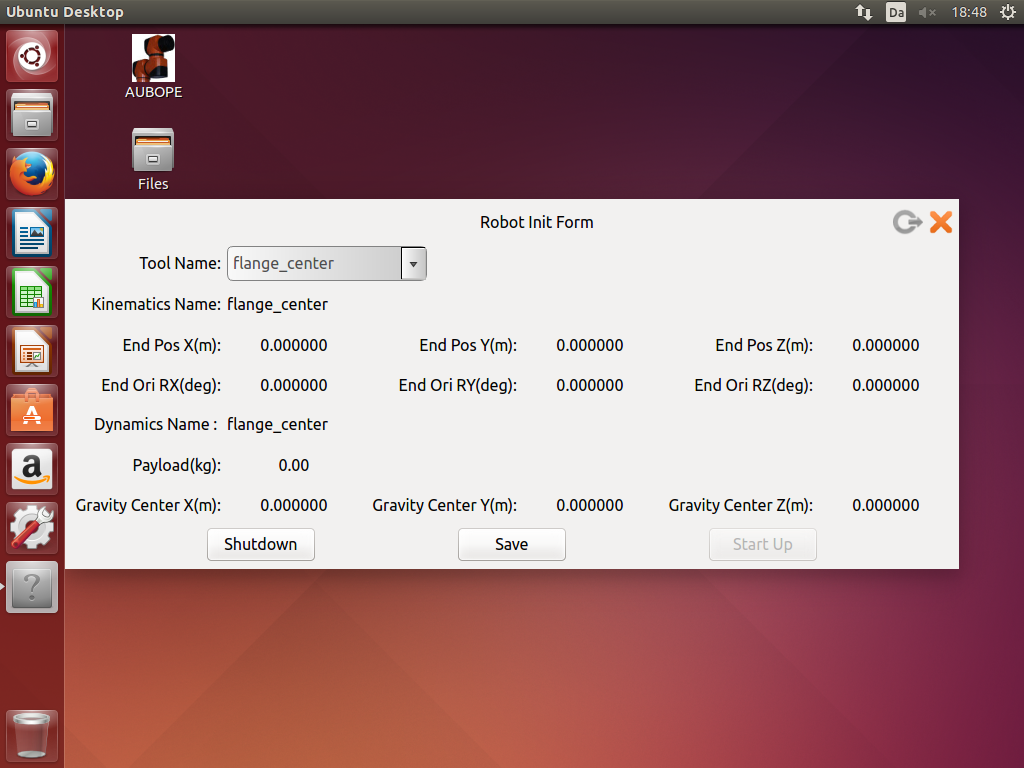
\includegraphics[width=0.8\textwidth]{../../Images/RobotInitForm.png}
\end{figure}
\item Press save and then startup to proceed.
\item Go to the about tab and in the top right
\item Check that the Teachpendant Version has been updated. An updated robot should say: Teachpendant Version: V4.5.49 
\end{enumerate}


\subsection{Installing Aubo Programs Using Backup File}
\label{subsec:usingBackup} 
With backups you can transfer all programs, variables and settings onto a new system. 
\begin{enumerate}
\item Acquire USB with backupfile and plug it into the robot.
\item Open AuboPE by double-clicking the shortcut on the desktop or by restarting the robot. The login screen should appear.
\begin{figure}[H]\centering
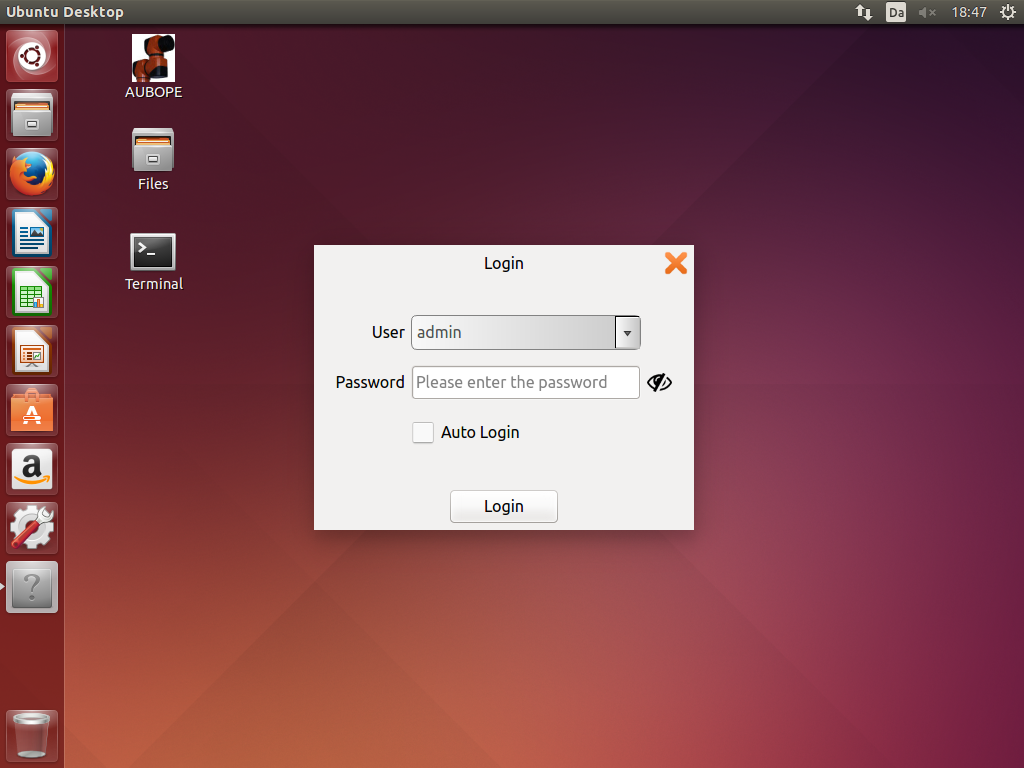
\includegraphics[width=0.8\textwidth]{../../Images/loginScreen.png}
\end{figure}
\item  Type the password, default is '1' and press login. The $Robot Init Form$ screen should appear
\begin{figure}[H]\centering
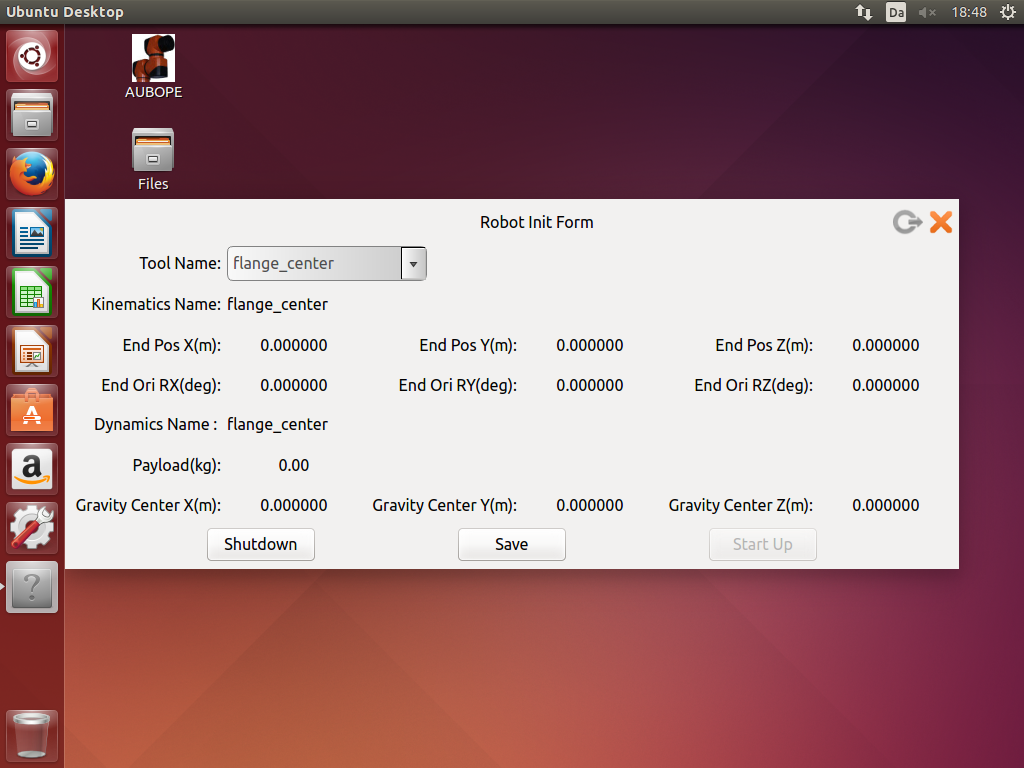
\includegraphics[width=0.8\textwidth]{../../Images/RobotInitForm.png}
\end{figure}
\item Press save and then startup to proceed.If this is the first time the robot has been started after being mounted it will say that the mounting pose has been changed. Click $ok$ and then click $yes$ to confirm that the mounting pose has changed. The robot will now initialize. You should hear the brakes click.  The teachpendant should then show the robot user interface.   
\item Click on the settings tab at the top. 
\begin{figure}[H]\centering
  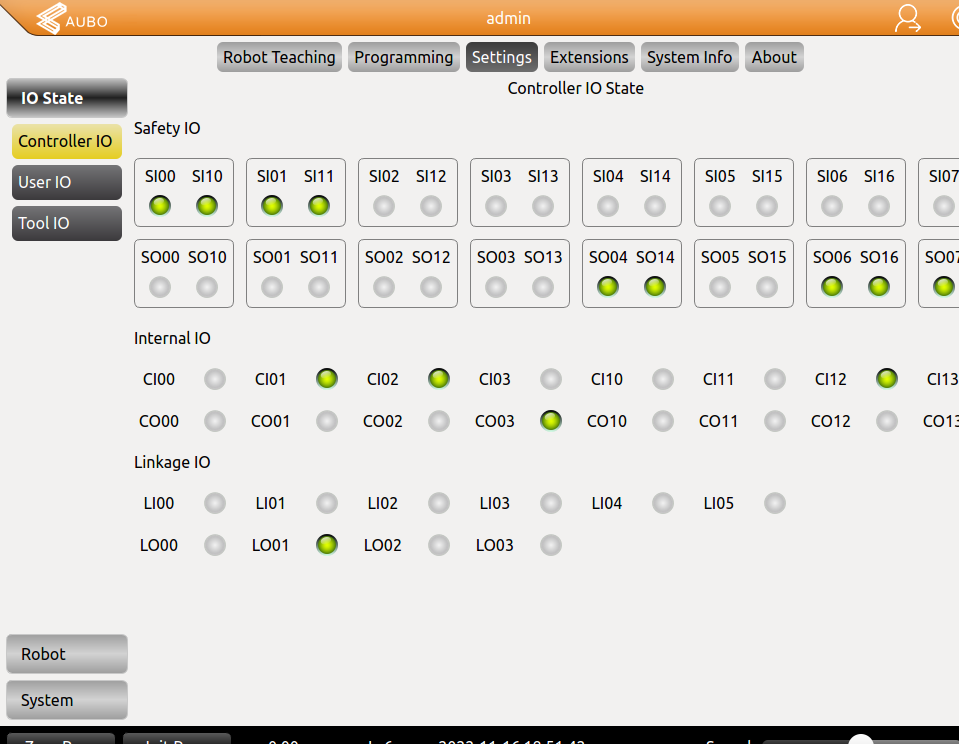
\includegraphics[width=0.8\textwidth]{../../Images/settings.png}
\end{figure}
\item Navigate through the $System$ tab into the $Update$ tab on the bottom left. 
\begin{figure}[H]\centering
  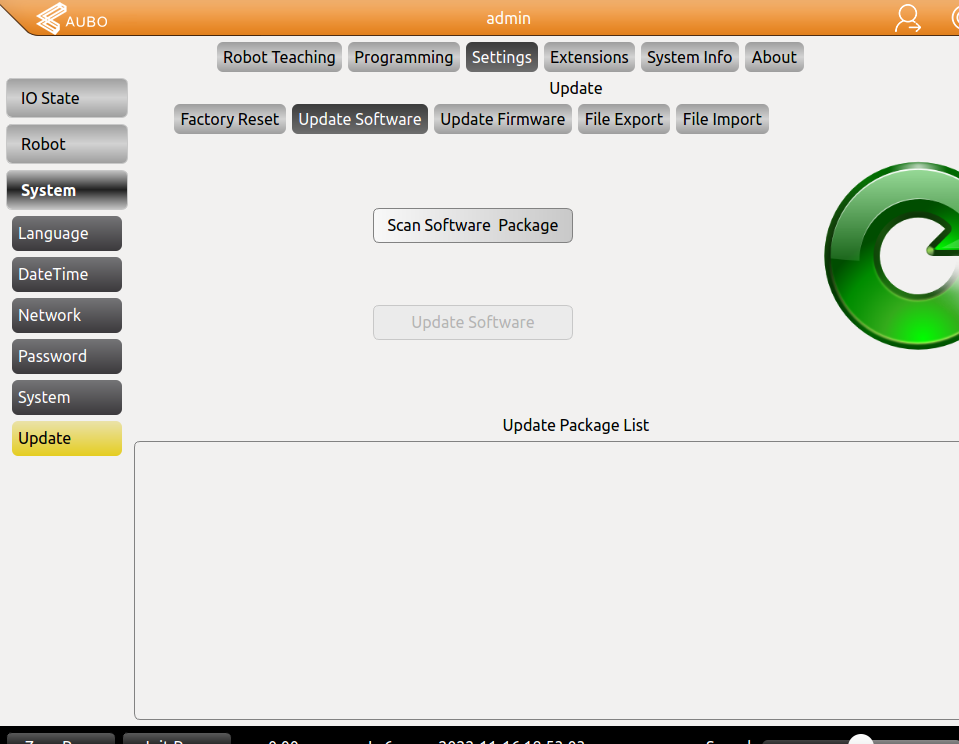
\includegraphics[width=0.8\textwidth]{../../Images/update.png}
\end{figure}
\item Select the $'File Import'$ tab.
\begin{figure}[H]\centering
  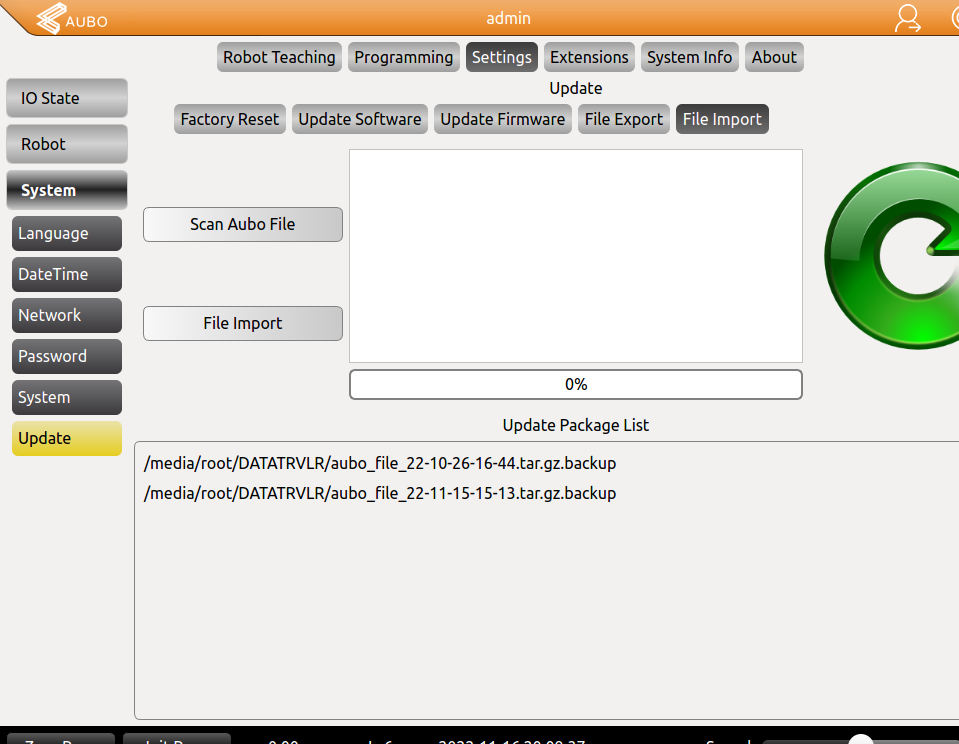
\includegraphics[width=0.8\textwidth]{../../Images/FileImport.png}
\end{figure}
\item Click $Scan Aubo File$. The path to any backup files on your USB should appear in the $Update Package List$
\item Select the desired backup and press $'File Import'$
\item Wait a moment for the backup to install. 
\item Restart the robot. Shutdown the robot by holding down the button on the teachpendant. Wait for the standby light to turn orange. Then press the teachpendant button again to start back up.
\end{enumerate}

\subsection{Tool pickup calibration} 
Becaus of imprecision in robot calibration, materials for the box or box assembly. The robot might not perform pickup of tools as smoothly as desired without a calibration of the pickup points. This section describes how to change those pickup points. 
The pickup point is defined as the moment we grab on to a tool. ie the moment we activate/deactivate the air in quickchange or 3D printed hand. 

\begin{enumerate}
\item Open AuboPE by double-clicking the shortcut on the desktop or by restarting the robot using the teachpendant power button. The login screen should appear.
\begin{figure}[H]\centering
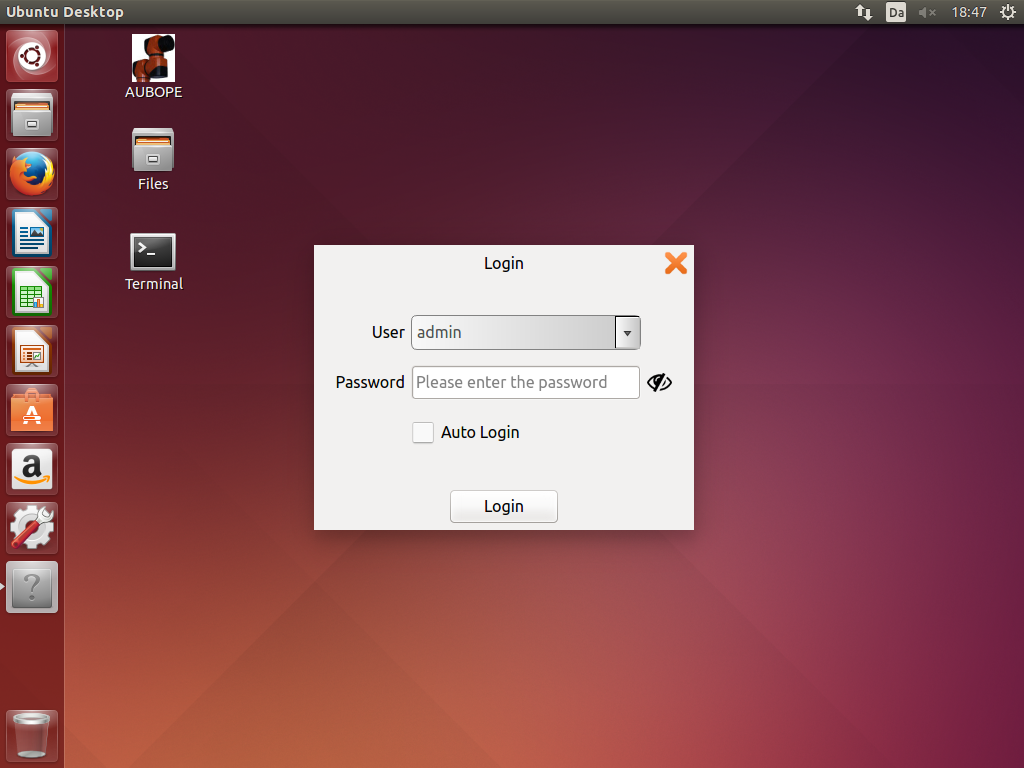
\includegraphics[width=0.8\textwidth]{../../Images/loginScreen.png}
\end{figure}
\item  Type the password, default is '1' and press login. The $Robot Init Form$ screen should appear
\begin{figure}[H]\centering
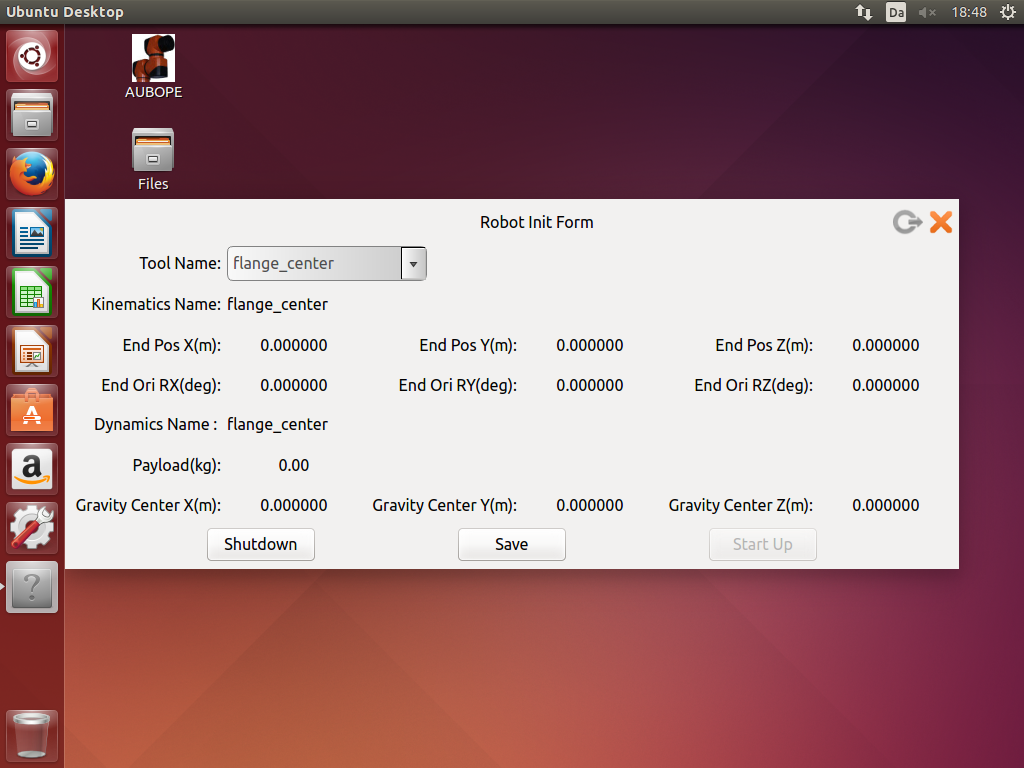
\includegraphics[width=0.8\textwidth]{../../Images/RobotInitForm.png}
\end{figure}
\item Press save and then startup to proceed.
\item Select the programming tab in the top.
\item Navigate through the $Config$ tab into the $Var Config$ tab on the left.
\item The variables on the right are the pickup poses of the robot named for the tool they pickup. The exception is connectionLost which is used for something else. 
\item Go through each tool variable and perform the following procedure. 
\begin{itemize}
\item Select the variable you want to calibrate on the right.
\item While being careful not to hit anything navigate to the current pickup position by holding the move here button in the button right. If you are about to collide with something let go of the move here button and use the black force control button on the right side of the teachpendant to pull the robot around the obstacle by hand.
\item When you get close to the pickup point you might have to stop using moveHere as the old pickup position could be wrong. Use the forcecontrol button and pull the robot into a better pickup position.
\item When you are at the right position press the setPoint button. 
\item Activate stepMode and move with the arrows to finetune your position.
\item Press confirm in the bottom right. 
\item Now press modify to save the changes. Your pickup point should now be modified. 
\end{itemize}
\item To test pickup positions go to programming tab in the top. 
\item Navigate through $Project$ tab on the left into $Load$ tab. 
\item On the right is a list of programs. The tooltests will be named as $<toolname>Test$ fx UVLightTest. 
\item select program click load
\item Make sure to move the robot free of any obstacles into the middle of the box. Also adjust the sliding bar called $move limit$ to reduce the speed the robot moves at. It is recommended to test a new calibration while moving slowly.
\item If your calibration was good the tool should now be picked up and sat back down without issue. If the pickup is still imprecise repeat the calibration. 
\end{enumerate}




\subsection{Changing Keyboard Layout}
The keyboard layout will normally be set to English(US). This might be fine but be aware, if you are using a different keyboard, that some keys might be placed differently. If you want to change the layout continue in this section.
\begin{enumerate}
\item start the robot and navigate to the desktop. If you are in the robot software there is a logout button in the top-right. 
\item Open a terminal, by double tapping the icon on the desktop. (or plug in a mouse and doubleclick on it)
\item Enter command: $unity\&$, beware if you haven't changed the keyboard layout the $\&$ sign will be on the key press $Shift+7$ as on a US keyboard not on a keypress of $Shift+6$ as with a Danish keyboard. This command will start the unity desktop environment and give you a toolbar on the left side of the screen.
\item Open system settings either on the toolbar to the left or with the dropdown menu in the topright corner of the screen. The icon is a gear and a wrench. 
\begin{figure}[H]\centering
  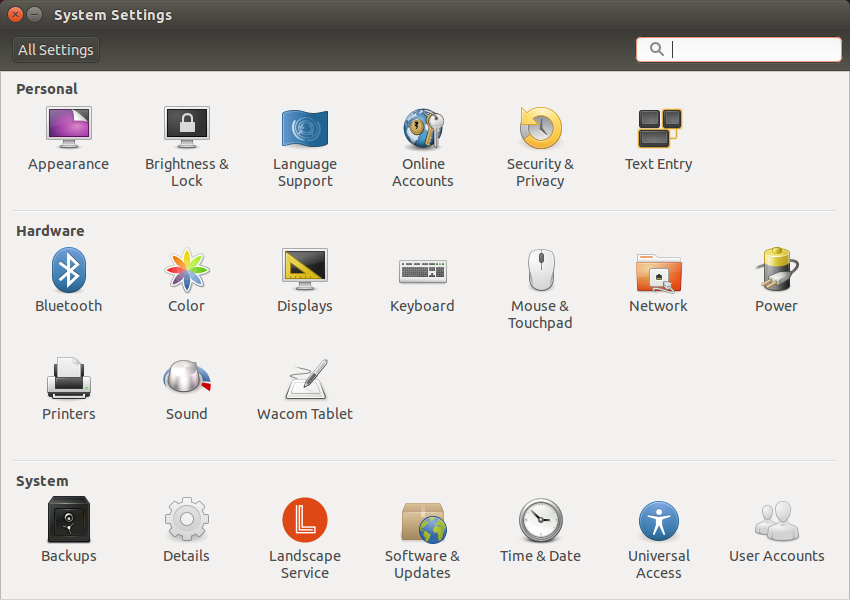
\includegraphics[width=0.8\textwidth]{../../Images/systemSettings.png}
\end{figure}
\item In system settings open ‘Text Entry’
\begin{figure}[H]\centering
  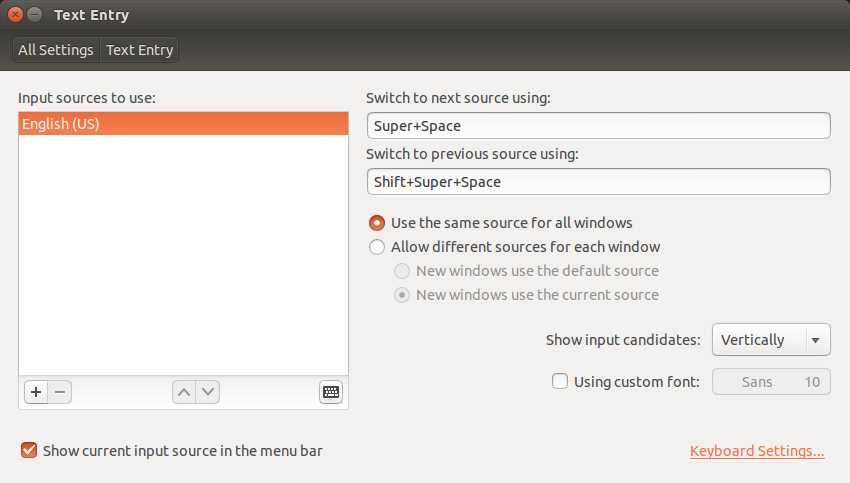
\includegraphics[width=0.8\textwidth]{../../Images/TextEntry.png}
\end{figure}
\item Under the list of input sources on the left press the ‘+’ button to add an input source. 
\item Find your desired layout in the list (fx. Danish). 
\begin{figure}[H]\centering
  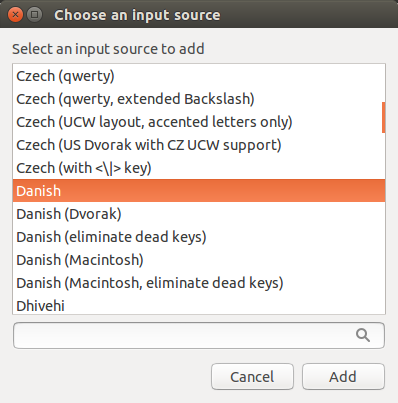
\includegraphics[width=0.8\textwidth]{../../Images/addingDanishLayout.png}
\end{figure}
\item Select your layout and press add. 
\item The name of your layout should now appear in the list of input sources marked with orange.
\begin{figure}[H]\centering
  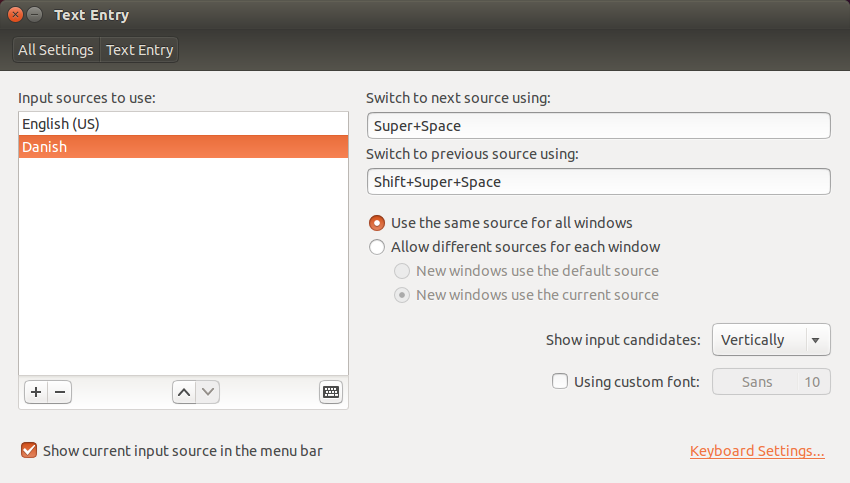
\includegraphics[width=0.8\textwidth]{../../Images/danishAddedToInputSources.png}
\end{figure}
\item Close the Text Entry box.
\item Go to the top right corner of the screen and click where it says ‘En’ for English. This will open a dropdown menu where you can now select your newly added keyboard layout.
\begin{figure}[H]\centering
  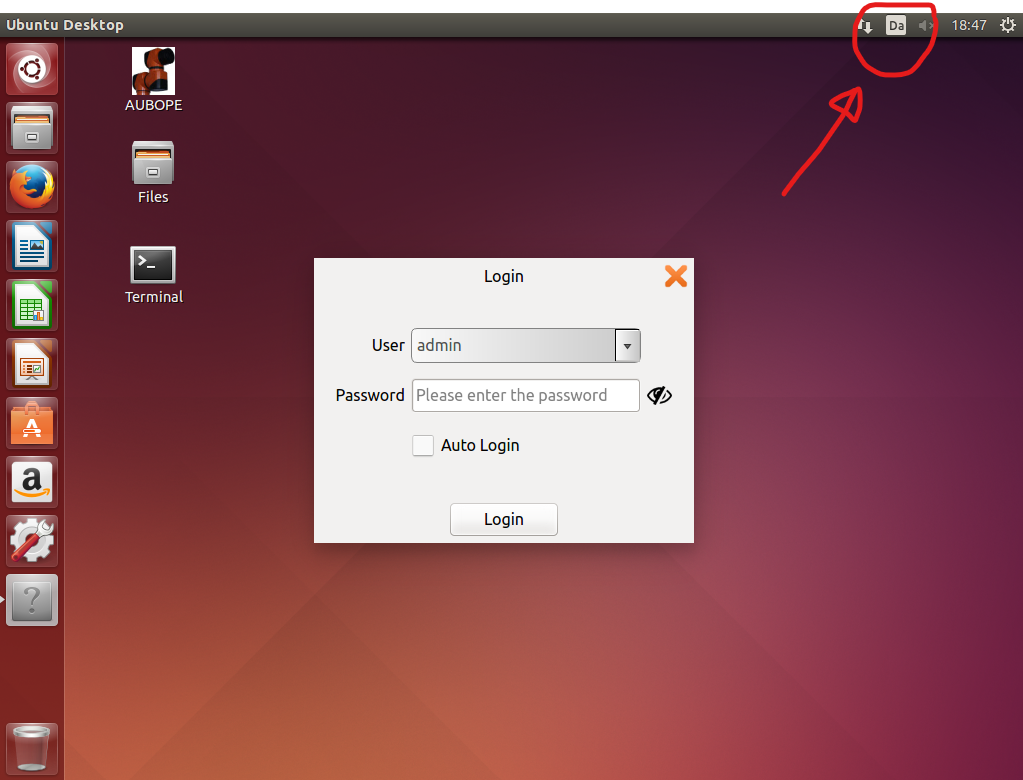
\includegraphics[width=0.8\textwidth]{../../Images/LanguageChange.png}
\end{figure} 
\item You should now have a different keyboard configuration. Test it by opening a terminal and typing some symbols.
\end{enumerate}

\subsection{Setting up remote Access with VNC and ssh}
Remote access means as long as you can get access to the local network you can open up the robot screen on your pc and send updates, and logs back and forth. 

\subsubsection{SSH}
To send files the SCP command is used. To be allowed access a tiny bit of setup is required. 
mainly you need to set a password. 
Open a terminal and type the command: $passwd$
Then type the desired password twice. Note what password you gave the machine. 

\subsubsection{VNC}
VNC is what lets us access the screen.
For this you are going to need access to the internet for the robot. It only does cable connection so get an ethernet cable and plug in your internet. Then follow instructions 
\href{https://tecadmin.net/setup-x11vnc-server-on-ubuntu-linuxmint/}{here}.

\subsection{Change IP using interfaces file}
Open a terminal and type the command $ifconfig$. 
This will list your connection. Find the name of your ethernet connection fx. $'eth3'$ and write out the ethernet specifications. An example could be. 
\#eth3
auto eth3 
iface eth3 inet static 
address 192.168.137.2 \#static Ip of robot
gateway 192.168.137.1 
netmask 255.255.255.0  
\#eth3 config finished
navigate to /etc/network/interfaces, and open it with a text editor. 
add your specification at the bottom of the file.
Now either restart the network config, or the entire system.

\subsection{Creating a Backup}
\begin{enumerate}
\item plugin a usb. 
\item Open AuboPE by double-clicking the shortcut on the desktop or by restarting the robot. The login screen should appear.
\begin{figure}[H]\centering
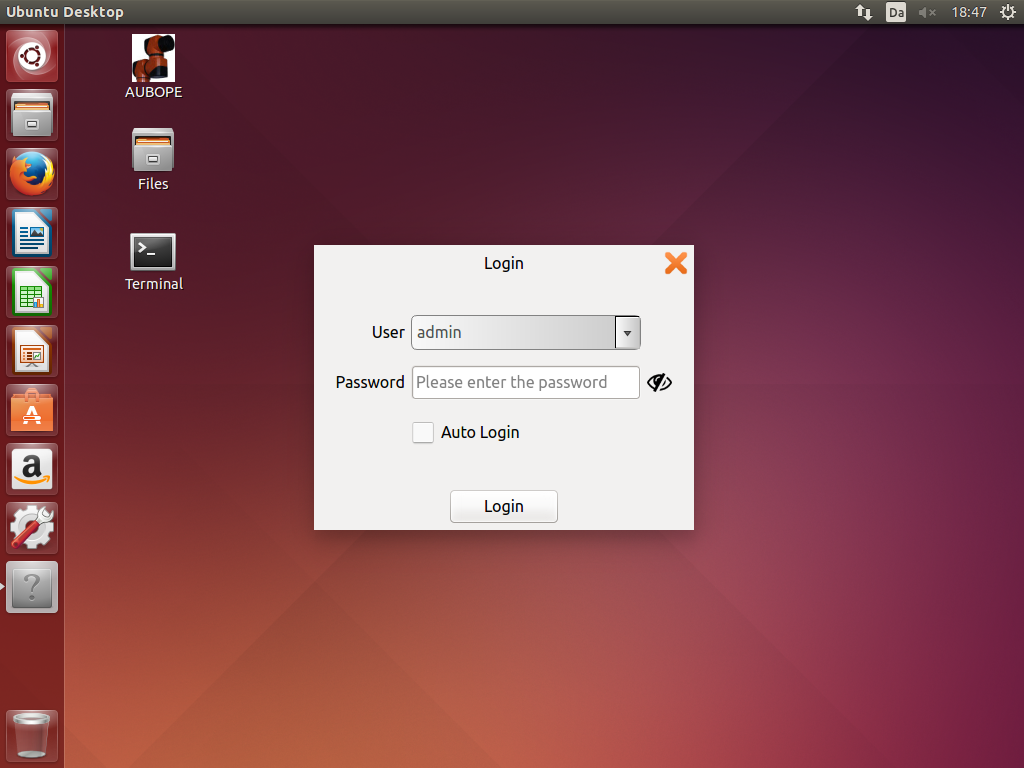
\includegraphics[width=0.8\textwidth]{../../Images/loginScreen.png}
\end{figure}
\item  Type the password, default is '1' and press login. The $Robot Init Form$ screen should appear
\begin{figure}[H]\centering
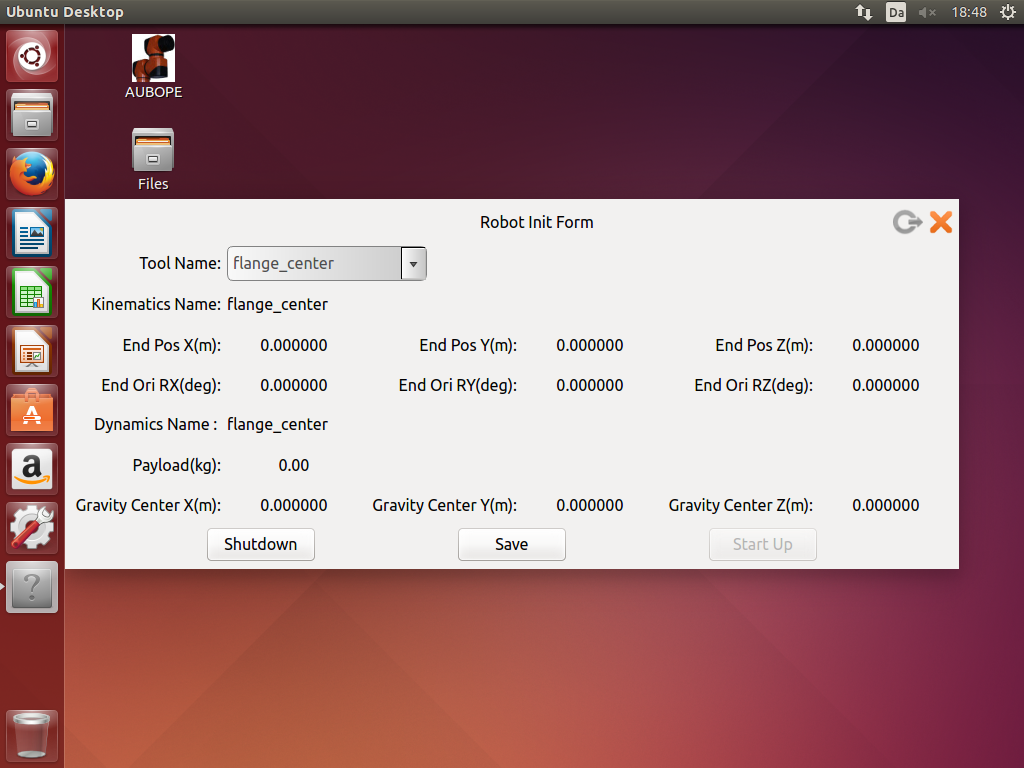
\includegraphics[width=0.8\textwidth]{../../Images/RobotInitForm.png}
\end{figure}
\item Press save and then startup to proceed.If this is the first time the robot has been started after being mounted it will say that the mounting pose has been changed. Click $ok$ and then click $yes$ to confirm that the mounting pose has changed. The robot will now initialize. You should hear the brakes click.  The teachpendant should then show the robot user interface. 
\item Click on the settings tab at the top. 
\begin{figure}[H]\centering
  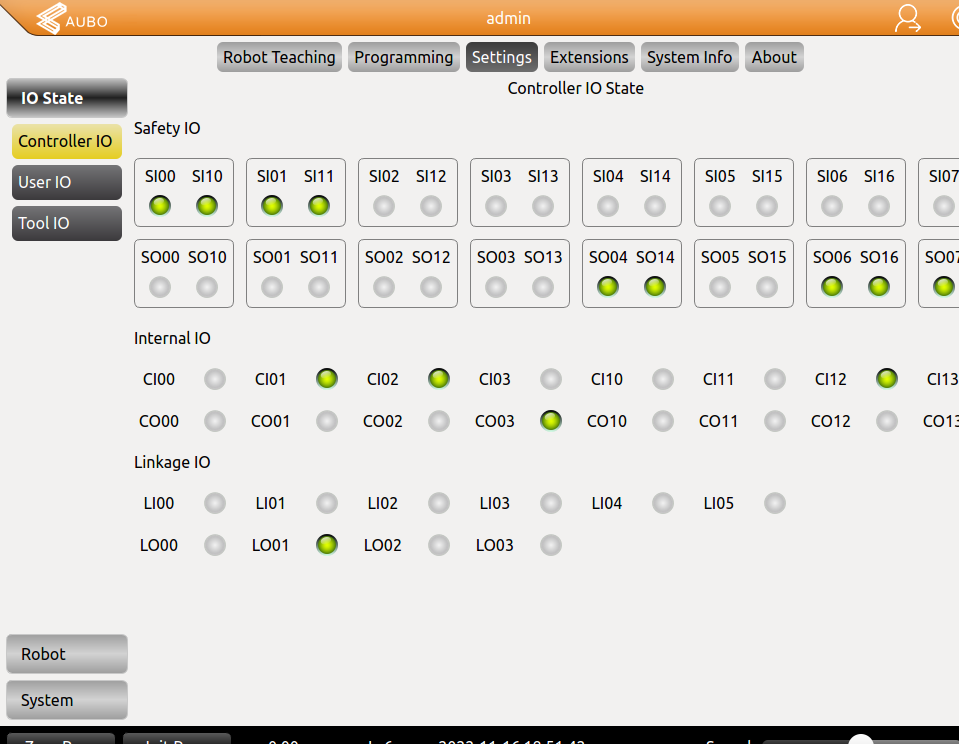
\includegraphics[width=0.8\textwidth]{../../Images/settings.png}
\end{figure}
\item Navigate through the $System$ tab into the $Update$ tab on the bottom left. 
\begin{figure}[H]\centering
  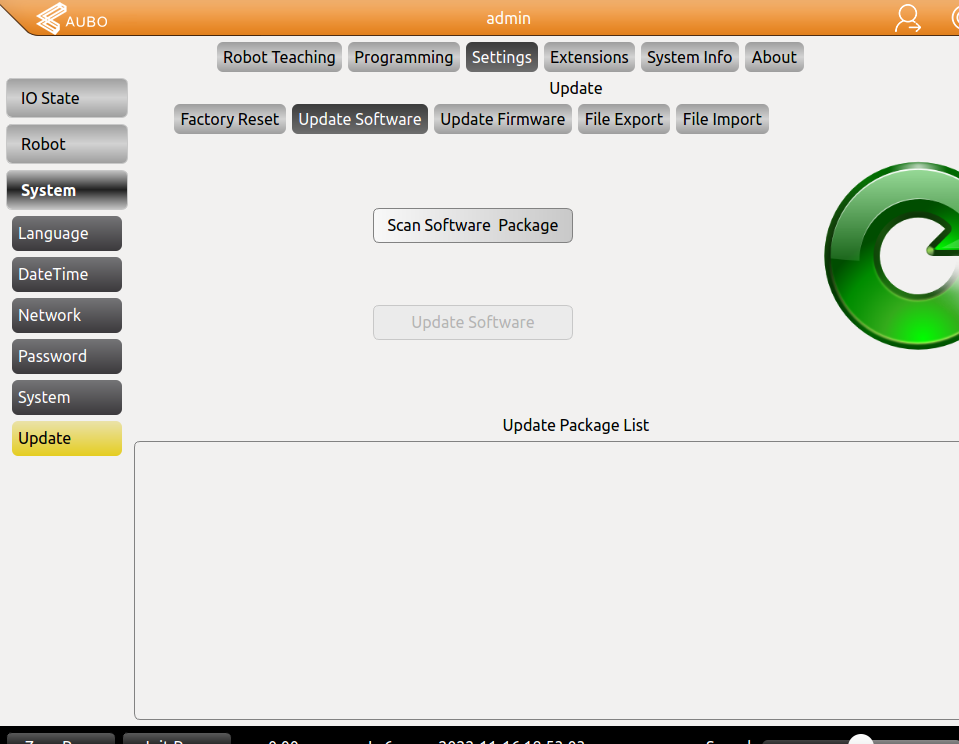
\includegraphics[width=0.8\textwidth]{../../Images/update.png}
\end{figure}
\item select the $'File Export'$ tab. 
\begin{figure}[H]\centering
  \includegraphics[width=0.8\textwidth]{../../Images/FileExport.png}
\end{figure}
\item click $'Scan Device'$. The path to your usb should appear in the $Update Package List$. 
\item Select your USB and then press $'File Export'$
\end{enumerate}


\subsection{Update manually}
Check out the guides \href{https://drive.google.com/drive/folders/1e2sAyCd5S1s4jH7FRyMwZzTy7VTZb2NE}{here}. For more info. 
 

\end{document}